%------------------------------%
%% ✎ Dylan (V1) %%%%%%%%% ✅ %%
%% ✎ Alain (V2) %%%%%%%%% ❌ %%
%% ✎ Dylan (V3) %%%%%%%%% ❌ %%
%------------------------------%

\afterpage{%
%\afterpage{%

    % Arrière-plan introduction generale
    \AddToShipoutPictureBG*{%
\includegraphics[width=\paperwidth,height=\paperheight]{src/Figures/Arriere_plan/Arriere_plan_Introduction.jpg}
    }

% Rectangle
\AddToShipoutPictureBG*{
  \begin{tikzpicture}[remember picture,overlay]
    \node[fill=white, opacity=0.75, text width=\paperwidth, minimum height=5cm, anchor=north] 
    at ([yshift=-9cm]current page.north) {};
  \end{tikzpicture}
}

% Source
\AddToShipoutPictureFG*{
  \AtPageLowerRight{
    \raisebox{1cm}{
      \hspace{16cm}
      
\begin{tikzpicture}
        \node[fill=white, rounded corners=5pt, inner sep=5pt, align=center] {
          \tiny{Photographie~: \textcolor{blue}{Dylan Moinse (2024)}}
        };
      \end{tikzpicture}
    }
  }
}
}%}

\renewcommand{\thefigure}{I.\arabic{figure}} % Numérotation spécifique pour l'introduction
\renewcommand{\thetable}{I.\arabic{table}}
\setcounter{figure}{0}

\pagenumbering{arabic}
\setcounter{page}{1} % Réinitialiser la numérotation à 1

    \needspace{1\baselineskip} % Réserve de l'espace
\part*{Introduction générale
    \label{body:introduction-generale}
    }
    %\addcontentsline{toc}{part}{Introduction générale}
    \markboth{Introduction générale}{}
    \markright{Introduction générale}{}
    \begin{refsegment}

    % Citation
    \begin{displayquote}
\Guillemets{\textsl{En gardant à l'esprit que~–~pour le même temps et effort~–~un individu peut parcourir à vélo une distance cinq fois supérieure à celle qu'il pourrait franchir à pied, ces aires de captation élargies jouent un rôle déterminant dans l'attraction d'une clientèle plus nombreuse vers le système de transport en commun. Ces zones peuvent également, dans une certaine mesure, modérer la demande immobilière aux abords des gares} [\dots] \textsl{Les investissements dans les infrastructures pour vélos, tels que les parkings et les services, sont économiquement rationnels pour les agences de transport public, augmentant à la fois la fréquentation du réseau et les revenus issus de son exploitation. Le vélo n'est plus perçu comme un concurrent, mais comme un allié, un moyen qui relie les voyageur·se·s à leur origine et à leur destination, et constitue un élément crucial d'un parcourus fluide de porte à porte. Ce type d'investissement collectif dans un système de transport en commun fréquent et flexible, visant à maximiser sa commodité et sa couverture spatiale, représente précisément l'action que les gouvernements doivent entreprendre pour alléger le fardeau financier associé à la possession d'une voiture et pour briser les barrières tangibles que rencontrent les individus les moins favorisés} [\dots] \textsl{Dans ce contexte, nous ne sommes plus contraint·e·s par la distance de marche nécessaire pour atteindre les commerces, les services et les nœuds~; nous n'avons plus à nous mesurer à la forte demande de cette proximité. Grâce à l'extension du rayon d'action permise en pédalant, nous avons pu soudainement étendre notre champ de recherche à de nouvelles parties de la ville} [\dots] \textsl{Une région équitable est celle qui garantit à tous ses résident·e·s un accès égal aux opportunités, indépendamment de leur origine géographique. Avec un réseau ferroviaire national et un réseau cyclable national, nous sommes assuré·e·s de pouvoir résider pratiquement où nous le souhaitons dans la Randstad, sans compromettre notre mode de vie ni nos opportunités d'emploi. Et pour nous, c'est un territoire où il fait bon vivre.}}\footnote{
    \Guillemets{\textsl{Keeping in mind that~–~for the same time and effort~–~someone can cycle five times farther than they can walk, these larger catchment areas actually play a critical role in feeding more customers into the public transport system. And they may~–~at least to a certain extent~–~tamp the demand for housing in and around train stations.} [\dots] \textsl{These investments in bicycle parking, rentals, and service make perfect economic sense for public transport agencies, as they increase ridership and revenue. Rather than treating the bicycle as a competitor, it is seen as an ally~–~one that connects passengers to their origin and destination; a critical component of the seamless door-to-door journey. These kinds of collective investments in a frequent and flexible public transport system~–~to maximize its convenience and coverage~–~are precisely what governments must do to lighten the financial burden of car ownership and break down the all-too-real barriers experienced by those lowest on the socioeconomic ladder.} [\dots] \textsl{in this case, we were no longer limited by the walking distance to shops, services, and public transport; nor were we forced to compete with the high demand for such proximity. With the extended range provided by pedal power, we could suddenly open up our search to entirely new parts of the city} [\dots] \textsl{An equitable region is one that provides residents with the same access to opportunity, regardless of their postal code. With a national rail network and national cycling network at our disposal, we know we can live virtually anywhere in the Randstad, without compromising on our lifestyle and our employment opportunities. And for us, that's a great place to be.}} \textcolor{blue}{\autocite[164-168]{bruntlett_curbing_2020}}\index{Bruntlett, Melissa|pagebf}\index{Bruntlett, Chris|pagebf}
} [traduction libre]%%Rédigé%%

\textcolor{blue}{\textcite{bruntlett_curbing_2020}}\index{Bruntlett, Melissa|pagebf}\index{Bruntlett, Chris|pagebf}. \foreignlanguage{english}{\textsl{Curbing Traffic: The Human Case for Fewer Cars in Our Lives}, Island Press, p. 164-168.}%%Rédigé%%
    \end{displayquote}

    % Amorce
\lettrine[lines=3, findent=8pt, nindent=0pt]{\lettrinefont R}{\textbf{emettre}} \textbf{la ville sur des rails}, tel est le message porté par l'anthropologie filmée, produite par \textcolor{blue}{Christian} \textcolor{blue}{\textcite{lallier_ville_2010}}\index{Lallier, Christian|pagebf}, anthropologue et réalisateur français. Intitulé \textsl{La ville sur des rails. L'utopie de la métropole}, ce documentaire explore les enjeux d'un urbanisme orienté vers le rail, remis au premier plan \textcolor{blue}{\autocite[8]{lhostis_concevoir_2009}}\index{L'Hostis, Alain|pagebf}\index{Alexandre, Elsa|pagebf}\index{Appert, Manuel|pagebf}\index{Araud-Ruyant, Catherine|pagebf}\index{Basty, Marius|pagebf}\index{Biau, Géraldine|pagebf}\index{Bozzani-Franc, Sandra|pagebf}\index{Boutantin, Gratienne|pagebf}\index{Constantin, Chantal|pagebf}\index{Coralli, Monica|pagebf}\index{Durousset, Marie-Jeanne|pagebf}\index{Fradier, Christophe|pagebf}\index{Gabion, Cyrille|pagebf}\index{Leysens, Thomas|pagebf}\index{Mermoud, Françoise|pagebf}\index{Olny, Xavier|pagebf}\index{Perrin, Emmanuel|pagebf}\index{Robert, Jean|pagebf}\index{Simand, Noémie|pagebf}\index{Stransky, Vaclav|pagebf}\index{Soulas, Claude|pagebf}\index{Verdier, Anne-Marie|pagebf}\index{Vulturescu, Bogdan|pagebf} dans une optique de réduction de la dépendance automobile \textcolor{blue}{\autocites[15]{newman_ten_2000}[74]{motte-baumvol_territoires_2014}[4]{gallez_dependance_2018}}\index{Motte-Baumvol, Benjamin|pagebf}\index{Belton-Chevallier, Leslie|pagebf}\index{Morel-Brochet, Annabelle|pagebf}\index{Gallez, Caroline|pagebf}\index{Newman, Peter W.~G.|pagebf}\index{Kenworthy, Jeffrey~R.|pagebf}. Les réflexions et les projets liés à la dialectique entre réseau et territoire, c'est-à-dire à l'articulation entre logiques territoriales et logiques réticulaires, connaissent un engouement récent \textcolor{blue}{\autocite[17]{gachon_impact_2019}}\index{Gachon, Mickaël|pagebf}, dans un contexte dans lequel leur coordination s'impose comme un incontournable des discours sur le \Guillemets{développement urbain \gls{durable}} \textcolor{blue}{\autocite[69]{nessi_politiques_2009}}\index{Nessi, Hélène|pagebf}\index{Delpirou, Aurélien|pagebf}, se traduisant principalement par une densification autour des gares. Ces auteur·rice·s soulèvent néanmoins des interrogations quant à la capacité systémique du rail à \Guillemets{corriger les anomalies} héritées de la fragmentation territoriale \textcolor{blue}{\autocite[190]{ducharme_ville_2021}}\index{Ducharme, Olivier|pagebf} et de la prégnance culturelle de l'\Guillemets{automobilité} \textcolor{blue}{\autocites[57-58]{urry_sociology_2000}[28]{urry_system_2004}}\index{Urry, John|pagebf}.%%Rédigé%%

    % Citation
Partant de ces critiques quant aux limites d'adaptabilité du \acrshort{TOD}, ou d'un urbanisme orienté vers les réseaux de \gls{transport en commun}, particulièrement dans les territoires dessinés par le système auto-centré, l'hypothèse directrice consiste à interroger le rôle stratégique du vélo et de la \gls{micro-mobilité}, qui présentent une tendance durable à un \Guillemets{retour en grâce} \textcolor{blue}{\autocites[137-168]{heran_retour_2015}[3-28]{dusong_dynamiques_2021}[44]{eskenazi_voir_2022}}\index{Héran, Frédéric|pagebf}\index{Dusong, Clément|pagebf}\index{Papon, Francis|pagebf}\index{Eskenazi, Manon|pagebf}\index{Massot, \index{Eskenazi, Manon|pagebf}|pagebf} ou font l'objet de réinventions \textcolor{blue}{\autocite[18]{amar_homo_2016}}\index{Amar, Georges|pagebf}. L'intérêt de cette recherche doctorale est d'évaluer dans quelle mesure ces modes de déplacement peuvent combler les lacunes du concept d'aménagement originellement formulé, en reconfigurant les interactions entre proximités, transport public et formes urbaines, dans une perspective intermodale. À cet égard, nous envisageons l'essor observé des cycles comme une opportunité pour répondre efficacement à la problématique des \Guillemets{premiers et derniers kilomètres} du transport public. Cette thèse explore à ce titre l'effet d'aubaine que représente l'émergence de nouvelles solutions de mobilité au sein de cette famille de véhicules individuels et légers \textcolor{blue}{\autocite[77]{oostendorp_combining_2018}}\index{Oostendorp, Rebekka|pagebf}\index{Gebhardt, Laura|pagebf}, afin de favoriser des parcours \Guillemets{fluides et porte-à-porte}, ainsi que le résume avec justesse la citation tirée de l'ouvrage de \textcolor{blue}{\textcite[164-168]{bruntlett_curbing_2020}}\index{Bruntlett, Melissa|pagebf}\index{Bruntlett, Chris|pagebf}.%%Résumé%%

% --- %
    % *.1. Contexte
    \needspace{1\baselineskip} % Réserve de l'espace
\section*{Regards croisés sur l’organisation territoriale et la mobilité spatiale
    \label{introduction-generale:regards-croises-organisation-territoriale-mobilite-spatiale}
    }
    \addcontentsline{toc}{section}{Regards croisés sur l’organisation territoriale et la mobilité spatiale}
    %\markboth{Regards croisés sur l’organisation territoriale et la mobilité spatiale}{}
    \markright{Regards croisés sur l’organisation territoriale et la mobilité spatiale}{}

    % Contexte
Le secteur des \Guillemets{transports} demeure le premier poste d'émission de \acrfull{GES} en France, en 2022, en représentant 32~\% du total des émissions nationales \textcolor{blue}{\autocite[41-53]{ministere_de_la_transition_ecologique_et_de_la_cohesion_des_territoires_chiffres_2024}}\index{Ministère de la Transition Écologique et de la Cohésion des Territoires@\textsl{Ministère de la Transition Écologique et de la Cohésion des Territoires}|pagebf}. Malgré une tendance générale à la réduction de l'empreinte carbone dans le territoire, le secteur des transports enregistre une augmentation de 2,3~\% de ses émissions carbonées sur une année. Cette hausse est essentiellement imputable à l'utilisation de la voiture individuelle, responsable de plus de la moitié de ces émissions, et ce, en dépit des promesses techniques et technologiques fréquemment mises en avant. L'usage décomplexé de l'\Guillemets{autosolisme} s'inscrit dans un cercle vicieux automobile, où la croissance urbaine européenne, depuis l'après-guerre, a été durablement façonnée par son adaptation à la généralisation de l'automobile. Ce processus a entraîné une fragmentation des espaces, un allongement des distances parcourues, ainsi qu'une structuration des réseaux, des formes urbaines et des usages, à l'origine de vulnérabilités territoriales. Dès lors, le paradigme de la \Guillemets{mobilité durable} ou de la \Guillemets{transition mobilitaire} et, plus largement, sa \Guillemets{décarbonation}, relèvent avant tout d'une affaire d'urbanisme \textcolor{blue}{\autocite{societe_francaise_des_urbanistes_decarbonation_2024}}\index{Société française des urbanistes@\textsl{Société française des urbanistes}|pagebf}. En ce sens, le quartier de gare constitue un point de jonction stratégique entre la ville et le transport, concentrant l'attention des aménageur·se·s. Pour \Guillemets{retisser} la ville, le transport public doit être envisagé comme l'élément structurant des corridors et des quartiers, un pivot à partir duquel les acteurs de la fabrique urbaine sont invités à repenser l'organisation des territoires \textcolor{blue}{\autocite[8]{boisclair_retisser_2013}}\index{Boisclair, Catherine|pagebf}.%%Rédigé%%

    % TOD
S’élevant au rang de référentiel d’action, la question de la coordination entre urbanisme et transport, au-delà du \Guillemets{mythe de la cohérence}, évoque le modèle théorique et opérationnel du \acrfull{TOD} \textcolor{blue}{\autocite[183-220]{gallez_mythes_2010}}\index{Gallez, Caroline|pagebf}\index{Kaufmann, Vincent|pagebf}\index{Guerrinha, Christophe|pagebf}\index{Maksim, Hanja-Niriana|pagebf}\index{Thébert, Mariane|pagebf}, dans lequel l’objet technique et son milieu interagissent en co-construction dans le temps \textcolor{blue}{\autocite[44-50]{leheis-guillot_ville_2011}}\index{Leheis-Guillot, Stéphanie|pagebf}. Cette démarche intégrée, qui consiste à penser simultanément la ville et le transport, repose sur un mécanisme d’interaction bidirectionnelle et continue, s’inscrivant dans une boucle de rétroaction \textcolor{blue}{\autocite[130]{wegener_overview_2004}}\index{Wegener, Michael|pagebf}. C’est dans ce cadre systémique que nous soutenons l’hypothèse selon laquelle le \acrshort{TOD} gagnerait à mieux intégrer les proximités générées par les quartiers de gare, tant en termes de polarisation des flux que d’opportunités d’insertion urbaine. À l’image du titre choisi par le chercheur britannique \textcolor{blue}{Rich~C.} \textcolor{blue}{\textcite[40]{mcilroy_this_2023}}\index{McIlroy, Rich~C.|pagebf}, dans son article \textsl{C'est là que les transports en commun montrent leurs limites}\footnote{
    \textsl{This is where public transport falls down} \textcolor{blue}{\autocite[40]{mcilroy_this_2023}}\index{McIlroy, Rich~C.|pagebf}.
}, le défi premier du \acrshort{TOD} aujourd’hui est moins d'améliorer la qualité des transports en commun et d'intensifier les activités humaines autour des pôles d'échange que de valoriser les cheminements vers et depuis ces nodosités. En somme, alors que les espoirs de décarbonation de la mobilité se concentrent sur le \Guillemets{triptyque magique}~–~composé de la voiture tantôt électrique, tantôt partagée, tantôt autonome et connectée~–, tout porte à croire que cette focalisation sur l’automobile, dont les effets rebonds et les nuisances persistantes sont sous-estimés, se révélera insuffisante. À l’inverse, il convient de miser sur la synergie entre la marche, le \gls{vélo} et le transport public, un \Guillemets{triptyque intermodal} plus à même de répondre aux défis contemporains de la mobilité urbaine et de l’aménagement des territoires \textcolor{blue}{\autocite[1]{soulas_triptyque_2021}}\index{Soulas, Claude|pagebf}.%%Rédigé%%

    % Mobilité individuelle légère + Sujet de recherche
Le modèle urbain du \acrshort{TOD} vise à articuler deux échelles de mobilité quotidienne distinctes~: d’une part, la mobilité métropolitaine et régionale, structurée par les réseaux de transport en commun, et d’autre part, la mobilité de proximité, qui privilégie autant que possible la marche et les cycles \textcolor{blue}{\autocites[81]{conesa_modelisation_2010}[124]{lo_feudo_scenario_2014}}\index{Lo Feudo, Fausto|pagebf}\index{Menerault, Philippe|pagebf}\index{L'Hostis, Alain|pagebf}\index{Festa, Demetrio Carmine|pagebf}\index{Conesa, Alexis|pagebf}\index{Paris, Didier|pagebf}. Or, au cours de la dernière décennie, le vélo et la micro-mobilité ont connu une diversification telle qu'ils tendent à s'\Guillemets{hybrider}, évoluant vers des objets de transport individuels et transportables \textcolor{blue}{\autocite[20]{amar_du_2012}}\index{Amar, Georges|pagebf}, à l'image de la \acrfull{TEP}, ou s'apparentant à des systèmes de transport public individuel \textcolor{blue}{\autocites[179]{amar_homo_2010}[4]{castex_prise_2017}}\index{Castex, Élodie|pagebf}\index{Frère, Séverine|pagebf}\index{Groux, Annette|pagebf}\index{Amar, Georges|pagebf}, à l'instar de la mobilité partagée. À travers des processus d’innovation porteurs de transformations socio-spatiales \textcolor{blue}{\autocite[89]{ageron_intermodalite-voyageurs_2013}}\index{Ageron, Pierre|pagebf}\index{Varlet, Jean|pagebf}, ce que nous dénommons \Guillemets{mobilité individuelle légère} s'imbrique dans le réseau de transport en commun, en tant qu'offre modale complémentaire. Ses usages intermodaux sont intrinsèquement liés aux dimensions temporelles et spatiales, nous conduisant à développer une réflexion nourrie par les références aux espaces, aux territoires et aux lieux \textcolor{blue}{\autocite[4]{sebban_complementarite_2003}}\index{Sebban, Annie-Claude|pagebf}\index{Motte, Alain|pagebf}. C’est à partir de ces considérations que nous avons établi notre sujet de recherche, ayant pour titre~:
    \begin{displayquote}
\textbf{Le modèle urbain du \textsl{Transit-Oriented Development} revisité par la mobilité individuelle légère émergente. Une investigation dans la région Hauts-de-France.}
    \end{displayquote}%%Rédigé%%

% --- %
    % *.2. Positionnement scientifique
    \needspace{1\baselineskip} % Réserve de l'espace
\section*{Positionnement scientifique
    \label{introduction-generale:positionnement-scientifique}
    }
    \addcontentsline{toc}{section}{Positionnement scientifique}
    %\markboth{Positionnement scientifique}{}
    \markright{Positionnement scientifique}{}

    % Gare
Cette thèse s’inscrit dans une approche aménagiste, mobilisant les éléments issus de la \Guillemets{fabrique urbaine} avec une entrée spécifique par la matérialité des espaces publics. À titre d'hypothèse générale, nous adoptons comme cadre d'analyse le concept d’\Guillemets{urbanisme des réseaux} ou de \Guillemets{ville des réseaux}, considérés comme des modèles explicatifs des transformations urbaines \textcolor{blue}{\autocite[]{dupuy_urbanisme_1991}}\index{Dupuy, Gabriel|pagebf}. Ce cadre repose sur le postulat selon lequel l’organisation territoriale, rendue possible par les réseaux, offre une multiplicité de connexions dont l’optimisation est une condition à son efficacité. À cet égard, la gare est envisagée comme un \Guillemets{objet territorial} \textcolor{blue}{\autocite[7]{moretti_interconnexion_1999}}\index{Moretti, Anna|pagebf}\index{Vacheret, Guy|pagebf}, un espace à l'interface des réseaux de transport et des dynamiques urbaines. Cette conception s’inscrit dans une tendance récente des études urbaines visant à réinterroger le rôle des gares dans la structuration de ville contemporaine, à un \Guillemets{retour des gares en thèse} \textcolor{blue}{\autocite[489]{delage_gare_2013}}\index{Delage, Aurélie|pagebf}. Loin d’être réduite à un simple point de connexion fonctionnelle, la gare est ici envisagée dans toute sa complexité en tant que \Guillemets{système-gare} \textcolor{blue}{\autocites[395]{le_bot_quel_2019}{le_bot_management_2020}}\index{Le Bot, Nils|pagebf}. Cette posture intègre ses dimensions spatiales, organisationnelles et symboliques, en reconnaissant son rôle structurant non seulement pour les réseaux de transport, mais aussi pour la production et l’organisation urbaines, ainsi que pour les modes de vie qui y sont attachés. Aussi, la lecture du sujet de recherche se veut-elle transcalaire \textcolor{blue}{\autocite[3]{knowles_transit_2019}}\index{Knowles, Richard~D.|pagebf}\index{Ferbrache, Fiona|pagebf}, favorisant l'emboîtement des échelles temporelles et scalaires~; depuis l’évolution foncière et économique jusqu'aux projets urbains~; depuis l’échelle locale du bâtiment-voyageur·se·s jusqu’aux dimensions régionales et (inter)nationales \textcolor{blue}{\autocites[13-14]{menerault_gares_2001}[238]{chapelon_transports_2016}}.%%Rédigé%%

    % Proximités
Cette réflexion sur la gare ne saurait être dissociée des mobilités qu’elle polarise. Dès lors, cette recherche engage un glissement d’analyse, passant de l’objet gare à celui des proximités géographiques qu’elle génère, en intégrant une réflexion sur la mobilité individuelle légère et son rôle dans la structuration des quartiers de gare. Ce changement de focale s’inscrit dans un changement paradigmatique plus large dans l’analyse des mobilités, auquel la gare participe activement \textcolor{blue}{\autocite[53]{leheis-guillot_ville_2011}}\index{Leheis-Guillot, Stéphanie|pagebf}. Ce \Guillemets{tournant de la mobilité} \textcolor{blue}{\autocites{sheller_new_2006}[8]{sheller_mobilizing_2016}[13]{randell_no_2020}}\index{Sheller, Mimi|pagebf}\index{Urry, John|pagebf}\index{Randell, Richard|pagebf} met l’accent sur la dimension relationnelle et systémique du \gls{déplacement}, au-delà d’une approche strictement infrastructurelle \textcolor{blue}{\autocite[14]{heran_retour_2015}}\index{Héran, Frédéric|pagebf}. Dans ce cadre, cette thèse se situe à l’intersection de plusieurs champs de recherche, croisant urbanisme, aménagement du territoire, géographie, sociologie et science des données, afin d’interroger la reconfiguration du \acrshort{TOD} sous l’effet des (nouvelles) proximités permises par l’intégration de la mobilité individuelle légère. Cette approche conduit à considérer cette mobilité comme un levier stratégique pour la réactualisation du \acrshort{TOD} dans des contextes urbains hérités du modèle auto-orienté \textcolor{blue}{\autocite[209]{heran_retour_2015}}\index{Héran, Frédéric|pagebf}. Elle s’inscrit ainsi dans une réflexion plus large sur le renouvellement des politiques de transport public et d’aménagement, face aux défis des \Guillemets{premiers et derniers kilomètres}. Elle met en avant l’opportunité que représente la mobilité individuelle légère pour promouvoir un système de mobilité multimodale et de type \Guillemets{porte-à-porte} \textcolor{blue}{\autocite[979]{lee_bicycle-based_2016}}\index{Lee, Jaeyeong|pagebf}\index{Choi, Keechoo|pagebf}\index{Leem, Yountaik|pagebf}.%%Rédigé%%

    % Positionnement
Cette recherche doctorale mobilise ainsi quatre entrées complémentaires pour structurer notre investigation~: (i) l’entrée par les objets techniques, en analysant le \Guillemets{système-gare} et les modes de déplacement associés~; (ii) l’entrée par les usages et les pratiques intermodales, en étudiant les comportements et stratégies modales des cyclo-voyageur·se·s~; (iii) l’entrée par l’\gls{accessibilité}, en mesurant les effets de la mobilité individuelle légère sur l'accessibilité~; et (iv) l’entrée par les systèmes urbains, en interrogeant les effets de la mobilité individuelle légère sur l'urbanisme ferroviaire. Ainsi, la gare ne peut être réduite à un objet purement socio-technique \textcolor{blue}{\autocite[]{joseph_villes_1999}}\index{Joseph, Isaac|pagebf}, mais doit également être envisagée comme un objet urbain, en tenant compte de son insertion territoriale, au-delà de l’échelle du bâtiment-voyageur·se·s ou de son environnement immédiat. Elle joue un rôle spatial, fonctionnel et symbolique, en étant à la fois une \Guillemets{scène} et une \Guillemets{actante} \textcolor{blue}{\autocite[5]{baron_gares_2016}}\index{Baron, Nacima|pagebf}\index{Roseau, Nathalie|pagebf}. Cette démarche permet ainsi d’explorer le potentiel de révision du \acrshort{TOD} à travers l’intégration de la mobilité individuelle légère. Elle propose une lecture renouvelée des quartiers de gare et de leur rôle dans l’organisation urbaine, tout en contribuant à la formalisation d’un modèle élargi~: un \acrfull{M-TOD}, ou un urbanisme orienté vers les réseaux de transport en commun et intégrant la mobilité individuelle légère.%%Rédigé%%

% --- %
    % *.3. Problématique / Objectifs
    \needspace{1\baselineskip} % Réserve de l'espace
\section*{Orientations de recherche
    \label{introduction-generale:problematique-objectifs-hypotheses}
    }
    \addcontentsline{toc}{section}{Orientations de recherche}
    %\markboth{Problématique, objectifs et hypothèses de recherche}{}
    \markright{Problématique, objectifs et hypothèses de recherche}{}

    % Problématique
Cette thèse vise ainsi à examiner les transformations du modèle \acrshort{TOD} sous l'angle de la mobilité individuelle légère, en adoptant une approche théorique, empirique et prospective pour déterminer et établir un cadre optimal pour l'\gls{accessibilité intermodale}. Notre questionnement central se pose de la manière suivante~:
    \begin{displayquote}
\textbf{Dans quelle mesure l'intégration de la mobilité individuelle légère peut-elle relever les défis des \Guillemets{premiers et derniers kilomètres} du transport public et contribuer à renforcer l'accessibilité intermodale des quartiers de gare des Hauts-de-France~?
\\
En quoi ces \Guillemets{proximités} reconfigurent-elles le modèle urbain du \textsl{Transit-Oriented Development} et ouvrent-elles la voie à un \textsl{Micromobility-friendly Transit-Oriented Development}, mieux adapté aux réalités urbaines et aux évolutions des pratiques de mobilité~?
\\
Quelles sont les conditions de mise en œuvre et les leviers d’action à mobiliser pour assurer une intégration optimale de la mobilité individuelle légère dans les stratégies d’aménagement et de transport~?}
    \end{displayquote}%%Rédigé%%

    % Objectifs
Ce questionnement guidera ainsi la structuration de notre recherche, en montrant comment la mobilité individuelle légère peut enrichir le modèle du \acrshort{TOD} et quelles implications en découlent pour la planification des mobilités et des territoires. Au cours de notre projet doctoral, nous développerons une démarche progressive en plusieurs étapes, conçue pour revisiter le \acrshort{TOD} à l'aune des proximités renouvelées par le développement de la mobilité individuelle légère. Chaque chapitre s’appuie sur un objectif de recherche, articulant une réflexion théorique et empirique sur les enjeux de l'accessibilité intermodale (voir le \hyperref[fig-introduction:objectifs-hypotheses]{schéma~\ref{fig-introduction:objectifs-hypotheses}}, page~\pageref{fig-introduction:objectifs-hypotheses}). Afin de structurer notre raisonnement, nous avons recours à la méthode du questionnement dite \acrfull{QQOQCCP}, qui nous permet de préciser les contours et les objectifs de notre recherche~:
        \begin{customitemize}
    \item \textsl{Quoi} et \textsl{Quand}~? ({\textcolor{blue}{\(O_1\)}\label{objectif-1}}). Le premier chapitre pose les bases conceptuelles et historiques du \acrshort{TOD} et des cycles, en identifiant leurs forces et leurs limites. Il s’agit d’introduire le caractère essentiel d’un \acrshort{M-TOD}, c’est-à-dire un modèle réactualisé prenant en compte cette composante intermodale~;
    \item \textsl{Par qui} et \textsl{Sur quoi}~? ({\textcolor{blue}{\(O_2\)}\label{objectif-2}}). Le deuxième chapitre vise à construire un cadre analytique en procédant à une revue des travaux scientifiques et techniques existants sur la mobilité individuelle légère, l’\gls{intermodalité} et la relecture du \acrshort{TOD}. Il met en perspective les expériences internationales et les nouvelles connaissances en matière d'intermodalité~;
    \item \textsl{Où} et \textsl{Avec quoi}~? ({\textcolor{blue}{\(O_3\)}\label{objectif-3}}). Le troisième chapitre mobilise des méthodes mixtes pour construire et analyser un matériau empirique dans un périmètre géographique défini. Il s'agit de définir, d'adapter et de mettre en relation des approches appropriées en vue de proposer une \Guillemets{enquête sur-mesure}~;
    \item \textsl{Qui} et \textsl{Combien}~? ({\textcolor{blue}{\(O_4\)}\label{objectif-4}}). Le quatrième chapitre vient mesurer et caractériser les pratiques intermodales, en s’intéressant aux profils des usager·ère·s qui associent l'usage de la mobilité individuelle légère et du transport public. Il s’agit de quantifier les flux et d’identifier les facteurs socio-démographiques et environnementaux qui influencent de tels choix modaux~;
    \item \textsl{Vers où} et \textsl{Pourquoi}~? ({\textcolor{blue}{\(O_5\)}\label{objectif-5}}). Le cinquième chapitre a pour objectif de mesurer et d'expliquer l'extension spatiale des quartiers de gare grâce à la mobilité individuelle légère. Il évalue les gains d'accessibilité à différentes échelles~;
    \item \textsl{Comment} et \textsl{En relation avec quoi}~? ({\textcolor{blue}{\(O_6\)}\label{objectif-6}}). Le dernier chapitre propose une formalisation conceptuelle et opérationnelle du \acrshort{M-TOD} en modélisant les conditions de sa mise en œuvre. Il s’agit de formuler des recommandations à destination des acteurs de la fabrique urbaine.
        \end{customitemize}%%Rédigé%%

    % Figure objectifs et hypothèses de recherche
    \begin{figure}[h!]\vspace*{4pt}
        \caption{Vue d'ensemble des objectifs et des hypothèses de recherche}
        \label{fig-introduction:objectifs-hypotheses}
        \centerline{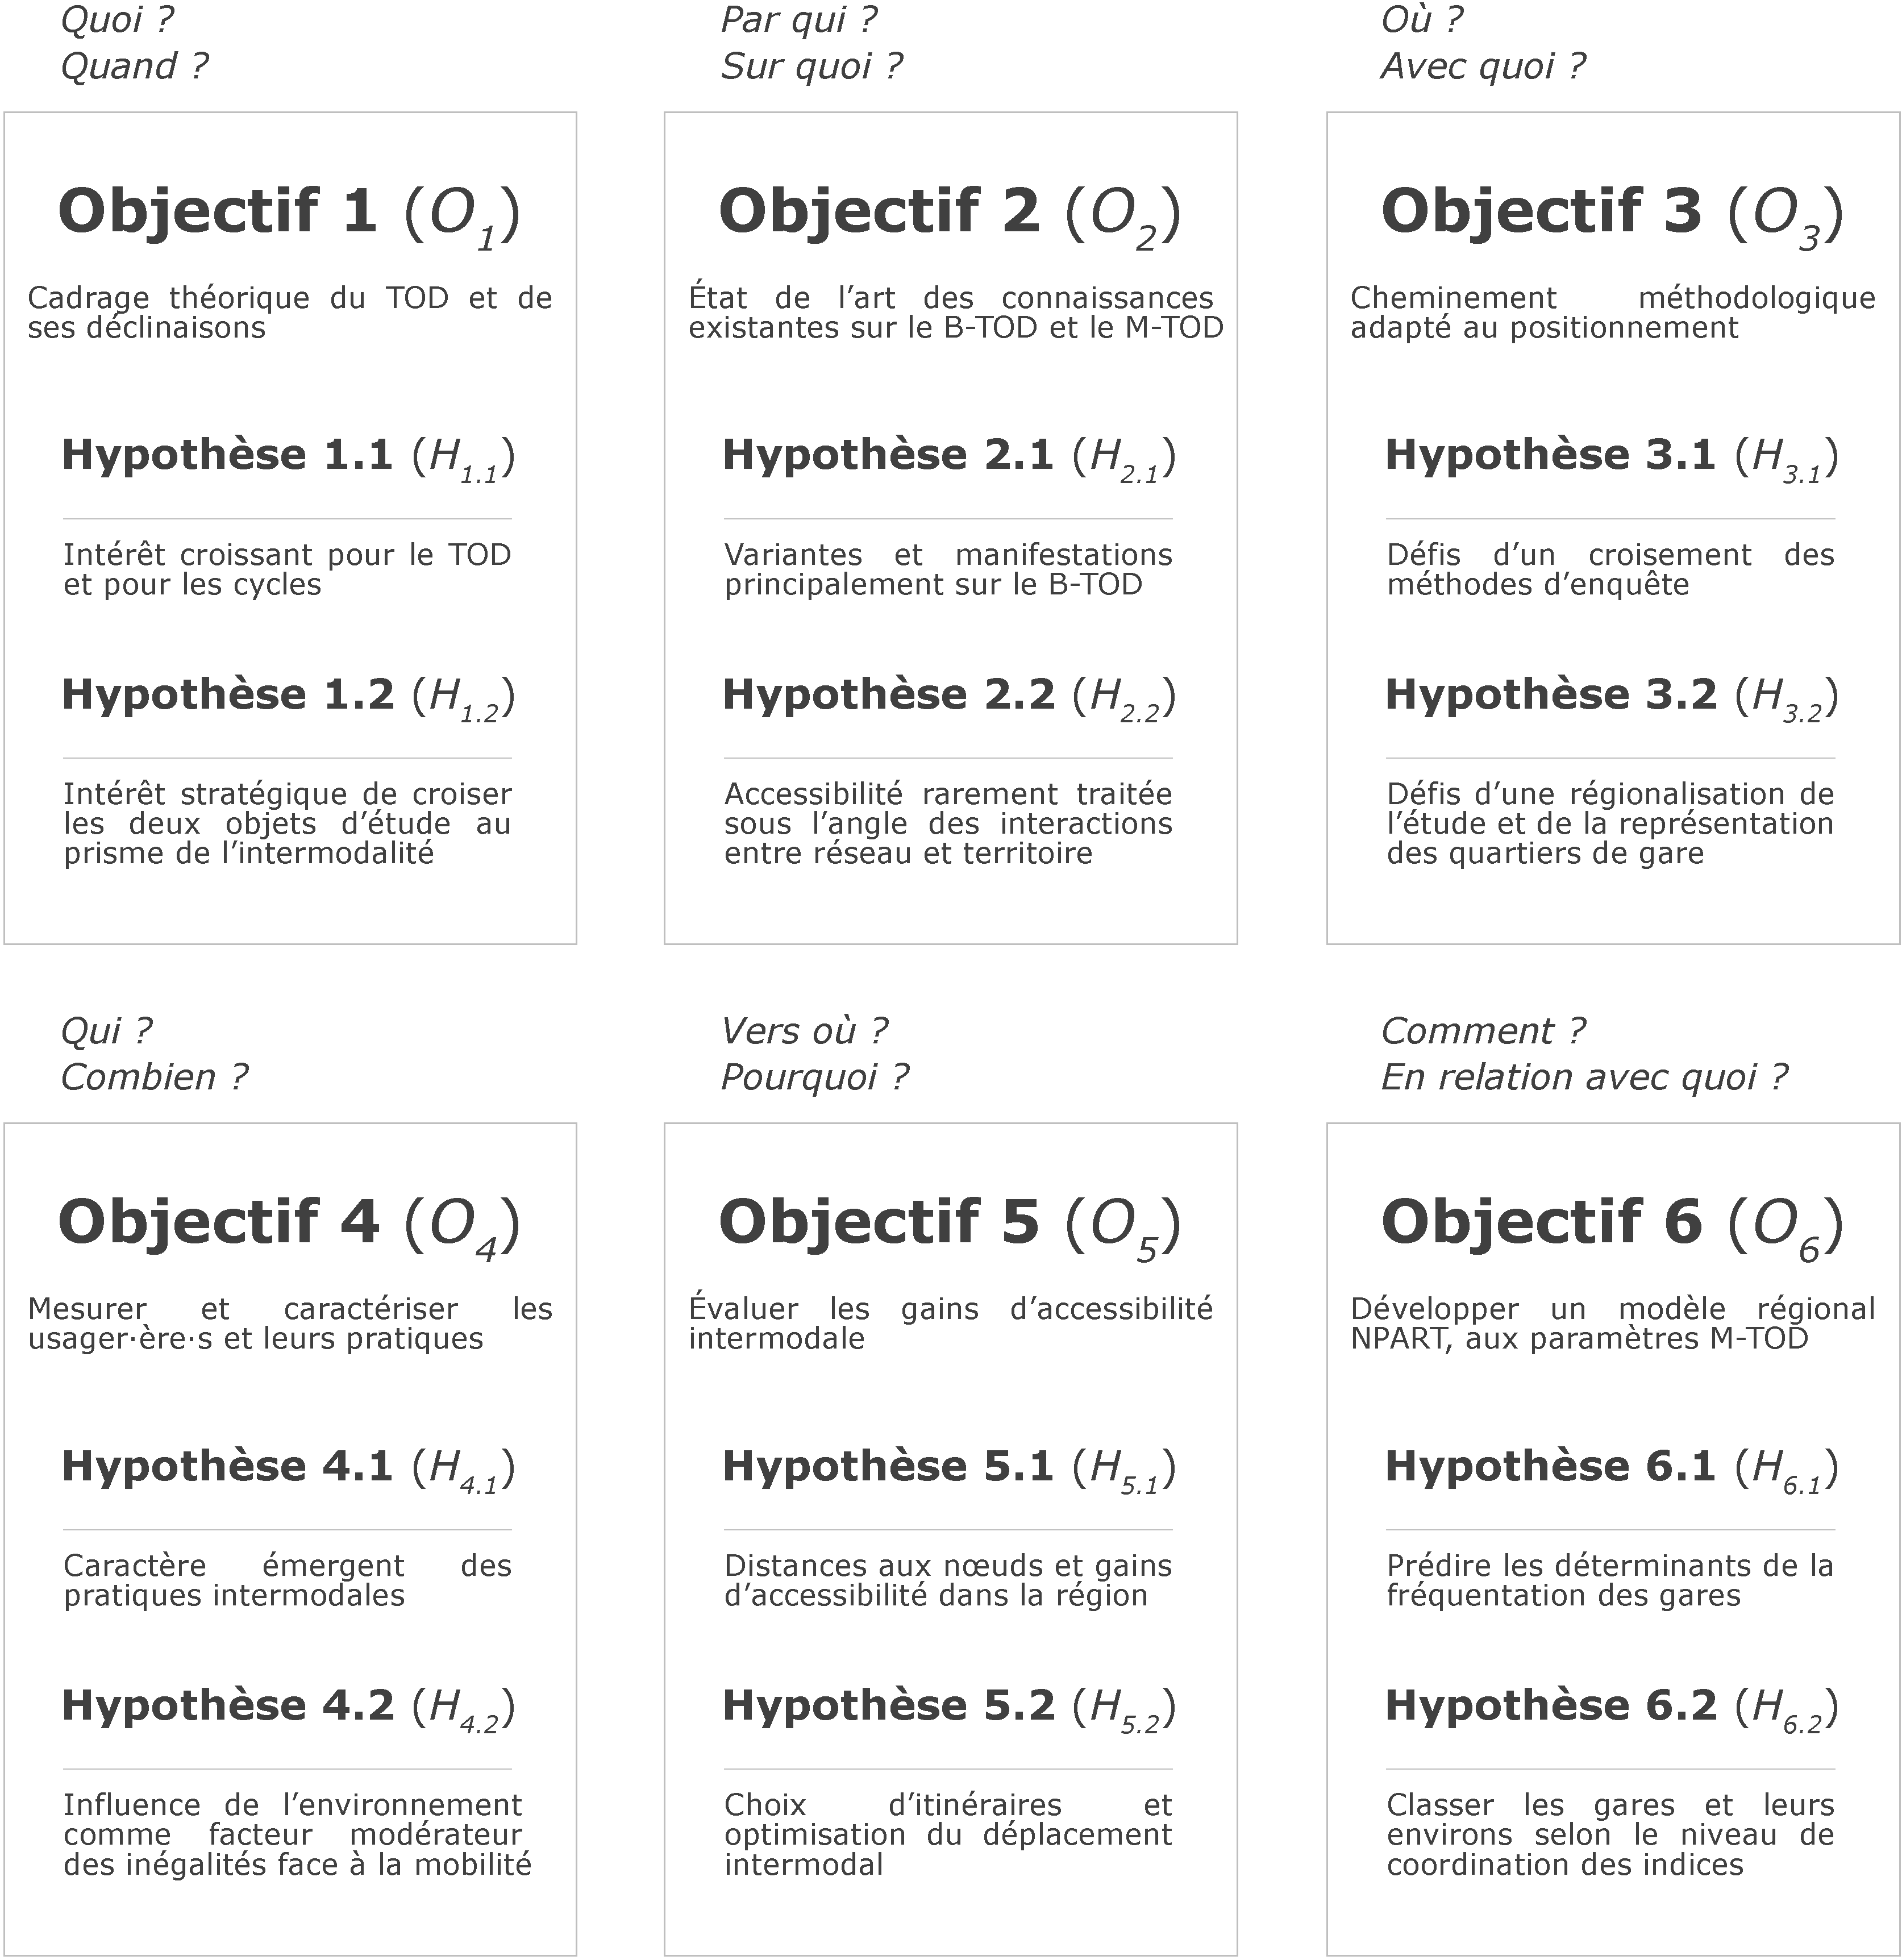
\includegraphics[width=1\columnwidth]{src/Figures/Introduction/FR_Objectifs_recherche.pdf}}
        \vspace{5pt}
        \begin{flushright}\scriptsize{
        Auteur~: \textcolor{blue}{Dylan Moinse (2023)}
        }\end{flushright}
    \end{figure}

    % Hypothèses
À partir des objectifs préalablement définis, lesquels structurent les différents chapitres de cette thèse, se dégagent les hypothèses de recherche qui constitueront le fil conducteur de notre démonstration tout au long de ce travail scientifique (voir le \hyperref[fig-introduction:objectifs-hypotheses]{schéma~\ref{fig-introduction:objectifs-hypotheses}}, page~\pageref{fig-introduction:objectifs-hypotheses}). Ces hypothèses s’inscrivent dans une démarche hypothético-déductive et se caractérisent par leur nature associative, complexe et directionnelle\footnote{
    Selon \textcolor{blue}{\textcite[41-43]{tomini_methodes_2020}}\index{Tomini, Luca|pagebf}\index{Wintgens, Sophie|pagebf}, dans leur manuel \textsl{Méthodes d'enquêtes de terrain en sciences sociales}, les hypothèses associatives postulent une relation d'interaction entre les concepts~; les hypothèses complexes, quant à elles, précisent une relation entre plusieurs concepts~; tandis que les hypothèses directionnelles formulent l'orientation des liens qui unit ces concepts.
} \textcolor{blue}{\autocite[43]{tomini_methodes_2020}}\index{Tomini, Luca|pagebf}\index{Wintgens, Sophie|pagebf}. En nous appuyant sur ces objectifs, nous proposons ainsi d’énoncer les hypothèses qui guideront notre réflexion~:
        \begin{customitemize}
    \item \textsl{Les thématiques de recherche émergentes relatives au \textsl{Transit-Oriented Development} et à la mobilité individuelle légère méritent d’être appréhendées de manière conjointe} ({\textcolor{blue}{\(H_1\)}\label{hypothese-1}}). En effet, ces deux axes suscitent un intérêt croissant tant dans les sphères académiques qu'opérationnelles ({\textcolor{blue}{\(S.H_{1.1}\)}\label{sous-hypothese-1.1}}) et gagneraient à être étudiés de manière articulée pour en révéler les synergies potentielles ({\textcolor{blue}{\(S.H_{1.2}\)}\label{sous-hypothese-1.2}})~;
    \item \textsl{Les connaissances actuelles relatives à cette synergie intermodale demeurent fortement conditionnées par le couple vélo et train, et sont rarement analysées au prisme du \textsl{Transit-Oriented Development}} ({\textcolor{blue}{\(H_2\)}\label{hypothese-2}}). En effet, les travaux existants se concentrent principalement sur l'objet vélo ({\textcolor{blue}{\(S.H_{2.1}\)}\label{sous-hypothese-2.1}}), tandis que les questions d’accessibilité sont majoritairement traitées sous l’angle strictement lié aux problématiques de transport ({\textcolor{blue}{\(S.H_{2.2}\)}\label{sous-hypothese-2.2}})~;
    \item \textsl{L’appréhension de la complexité des dynamiques intermodales et de leurs implications sur l’environnement urbain se heurte à la difficulté de définir une méthodologie d’analyse} ({\textcolor{blue}{\(H_3\)}\label{hypothese-3}}). Face aux lacunes identifiées dans la littérature, il apparaît pertinent de mobiliser une approche méthodologique mixte, combinant diverses méthodes d’enquête ({\textcolor{blue}{\(S.H_{3.1}\)}\label{sous-hypothese-3.1}}). De surcroît, l’adoption d’un périmètre d’étude à l’échelle régionale et la redéfinition de la notion de quartier de gare, en adéquation avec les principes du \acrshort{TOD}, s’imposent comme des ajustements nécessaires ({\textcolor{blue}{\(S.H_{3.2}\)}\label{sous-hypothese-3.2}})~;
    \item \textsl{Les pratiques intermodales connaissent un essor significatif sous l’effet conjugué de l’émergence de nouvelles solutions de mobilité, même si celles-ci sont marquées par une appropriation différenciée par divers groupes sociaux} ({\textcolor{blue}{\(H_4\)}\label{hypothese-4}}). Le développement de l’intermodalité intégrant les cycles et le transport public s’inscrit dans un processus de diversification et d'appropriation des modes de déplacement ({\textcolor{blue}{\(S.H_{4.1}\)}\label{sous-hypothese-4.1}}). Toutefois, cette appropriation reste inégale, certains groupes sociaux s’en saisissant plus aisément que d’autres, une situation qui pourrait néanmoins être atténuée par des interventions en matière d’aménagement du territoire ({\textcolor{blue}{\(S.H_{4.2}\)}\label{sous-hypothese-4.2}})~;
    \item \textsl{L’intégration de la mobilité individuelle légère au sein des réseaux de transport en commun constitue un levier majeur d’amélioration de l’accessibilité régionale} ({\textcolor{blue}{\(H_5\)}\label{hypothese-5}}). En effet, cette intégration permet d’accroître la portée des déplacements, étendant ainsi les périmètres de desserte des quartiers de gare et facilitant l’accès aux destinations ({\textcolor{blue}{\(S.H_{5.1}\)}\label{sous-hypothese-5.1}}). De plus, elle favorise l’optimisation des itinéraires, rendant les déplacements intermodaux plus compétitifs face à l’usage de l’automobile, y compris en ce qui concerne les mobilités quotidiennes de longue distance ({\textcolor{blue}{\(S.H_{5.2}\)}\label{sous-hypothese-5.2}})~;
    \item \textsl{L’élargissement du concept d’aménagement à la mobilité individuelle légère constitue un levier de dynamisation des quartiers de gare, en renforçant leur accessibilité dans une acception élargie} ({\textcolor{blue}{\(H_6\)}\label{hypothese-6}}). Certains facteurs liés à la cyclabilité des quartiers de gare contribuent à stimuler la demande autour des pôles d’échange ({\textcolor{blue}{\(S.H_{6.1}\)}\label{sous-hypothese-6.1}}), tout en les rendant plus cohérents avec les principes directeurs du \acrshort{TOD} ({\textcolor{blue}{\(S.H_{6.2}\)}\label{sous-hypothese-6.2}}).
\end{customitemize}%%Rédigé%%

% --- %
    % *.4. Méthodologie
    \needspace{1\baselineskip} % Réserve de l'espace
\section*{Stratégie de recherche
    \label{introduction-generale:methodologie}
    }
    \addcontentsline{toc}{section}{Stratégie de recherche}
    %\markboth{Méthodologie}{}
    \markright{Cadre méthodologique}{}

    % Introduction
Afin de répondre à la problématique de cette recherche ainsi qu’aux objectifs et hypothèses formulés, cette thèse adopte un dispositif méthodologique mixte, combinant des méthodes originales et adaptées aux spécificités du sujet étudié (voir le \hyperref[fig-introduction:methodes-hypotheses]{schéma~\ref{fig-introduction:methodes-hypotheses}}, page~\pageref{fig-introduction:methodes-hypotheses}). Cette démarche méthodologique permet d’articuler trois dimensions essentielles~: (i) une réflexion conceptuelle sur l’évolution du \acrshort{TOD} et son articulation avec la mobilité individuelle légère~; (ii) une investigation sur les pratiques intermodales existantes et les facteurs influençant ces comportements de mobilité~; et (iii) une évaluation des effets de la mobilité individuelle légère sur l’accessibilité aux gares et sur la structuration des quartiers environnants, dans un périmètre régional. Loin de constituer une approche linéaire, ce cheminement méthodologique assume sa complexité, mobilisant des outils complémentaires afin de saisir les multiples dimensions du \acrshort{TOD} et de la mobilité individuelle légère, conformément à l'\hyperref[hypothese-3]{hypothèse~\(H_3\)} (page~\pageref{hypothese-3}).%%Rédigé%%

    % Figure méthodologie hypothèses
    \begin{figure}[h!]\vspace*{4pt}
        \caption{Cadre méthodologique pensé en dialogue avec les hypothèses de recherche}
        \label{fig-introduction:methodes-hypotheses}
        \centerline{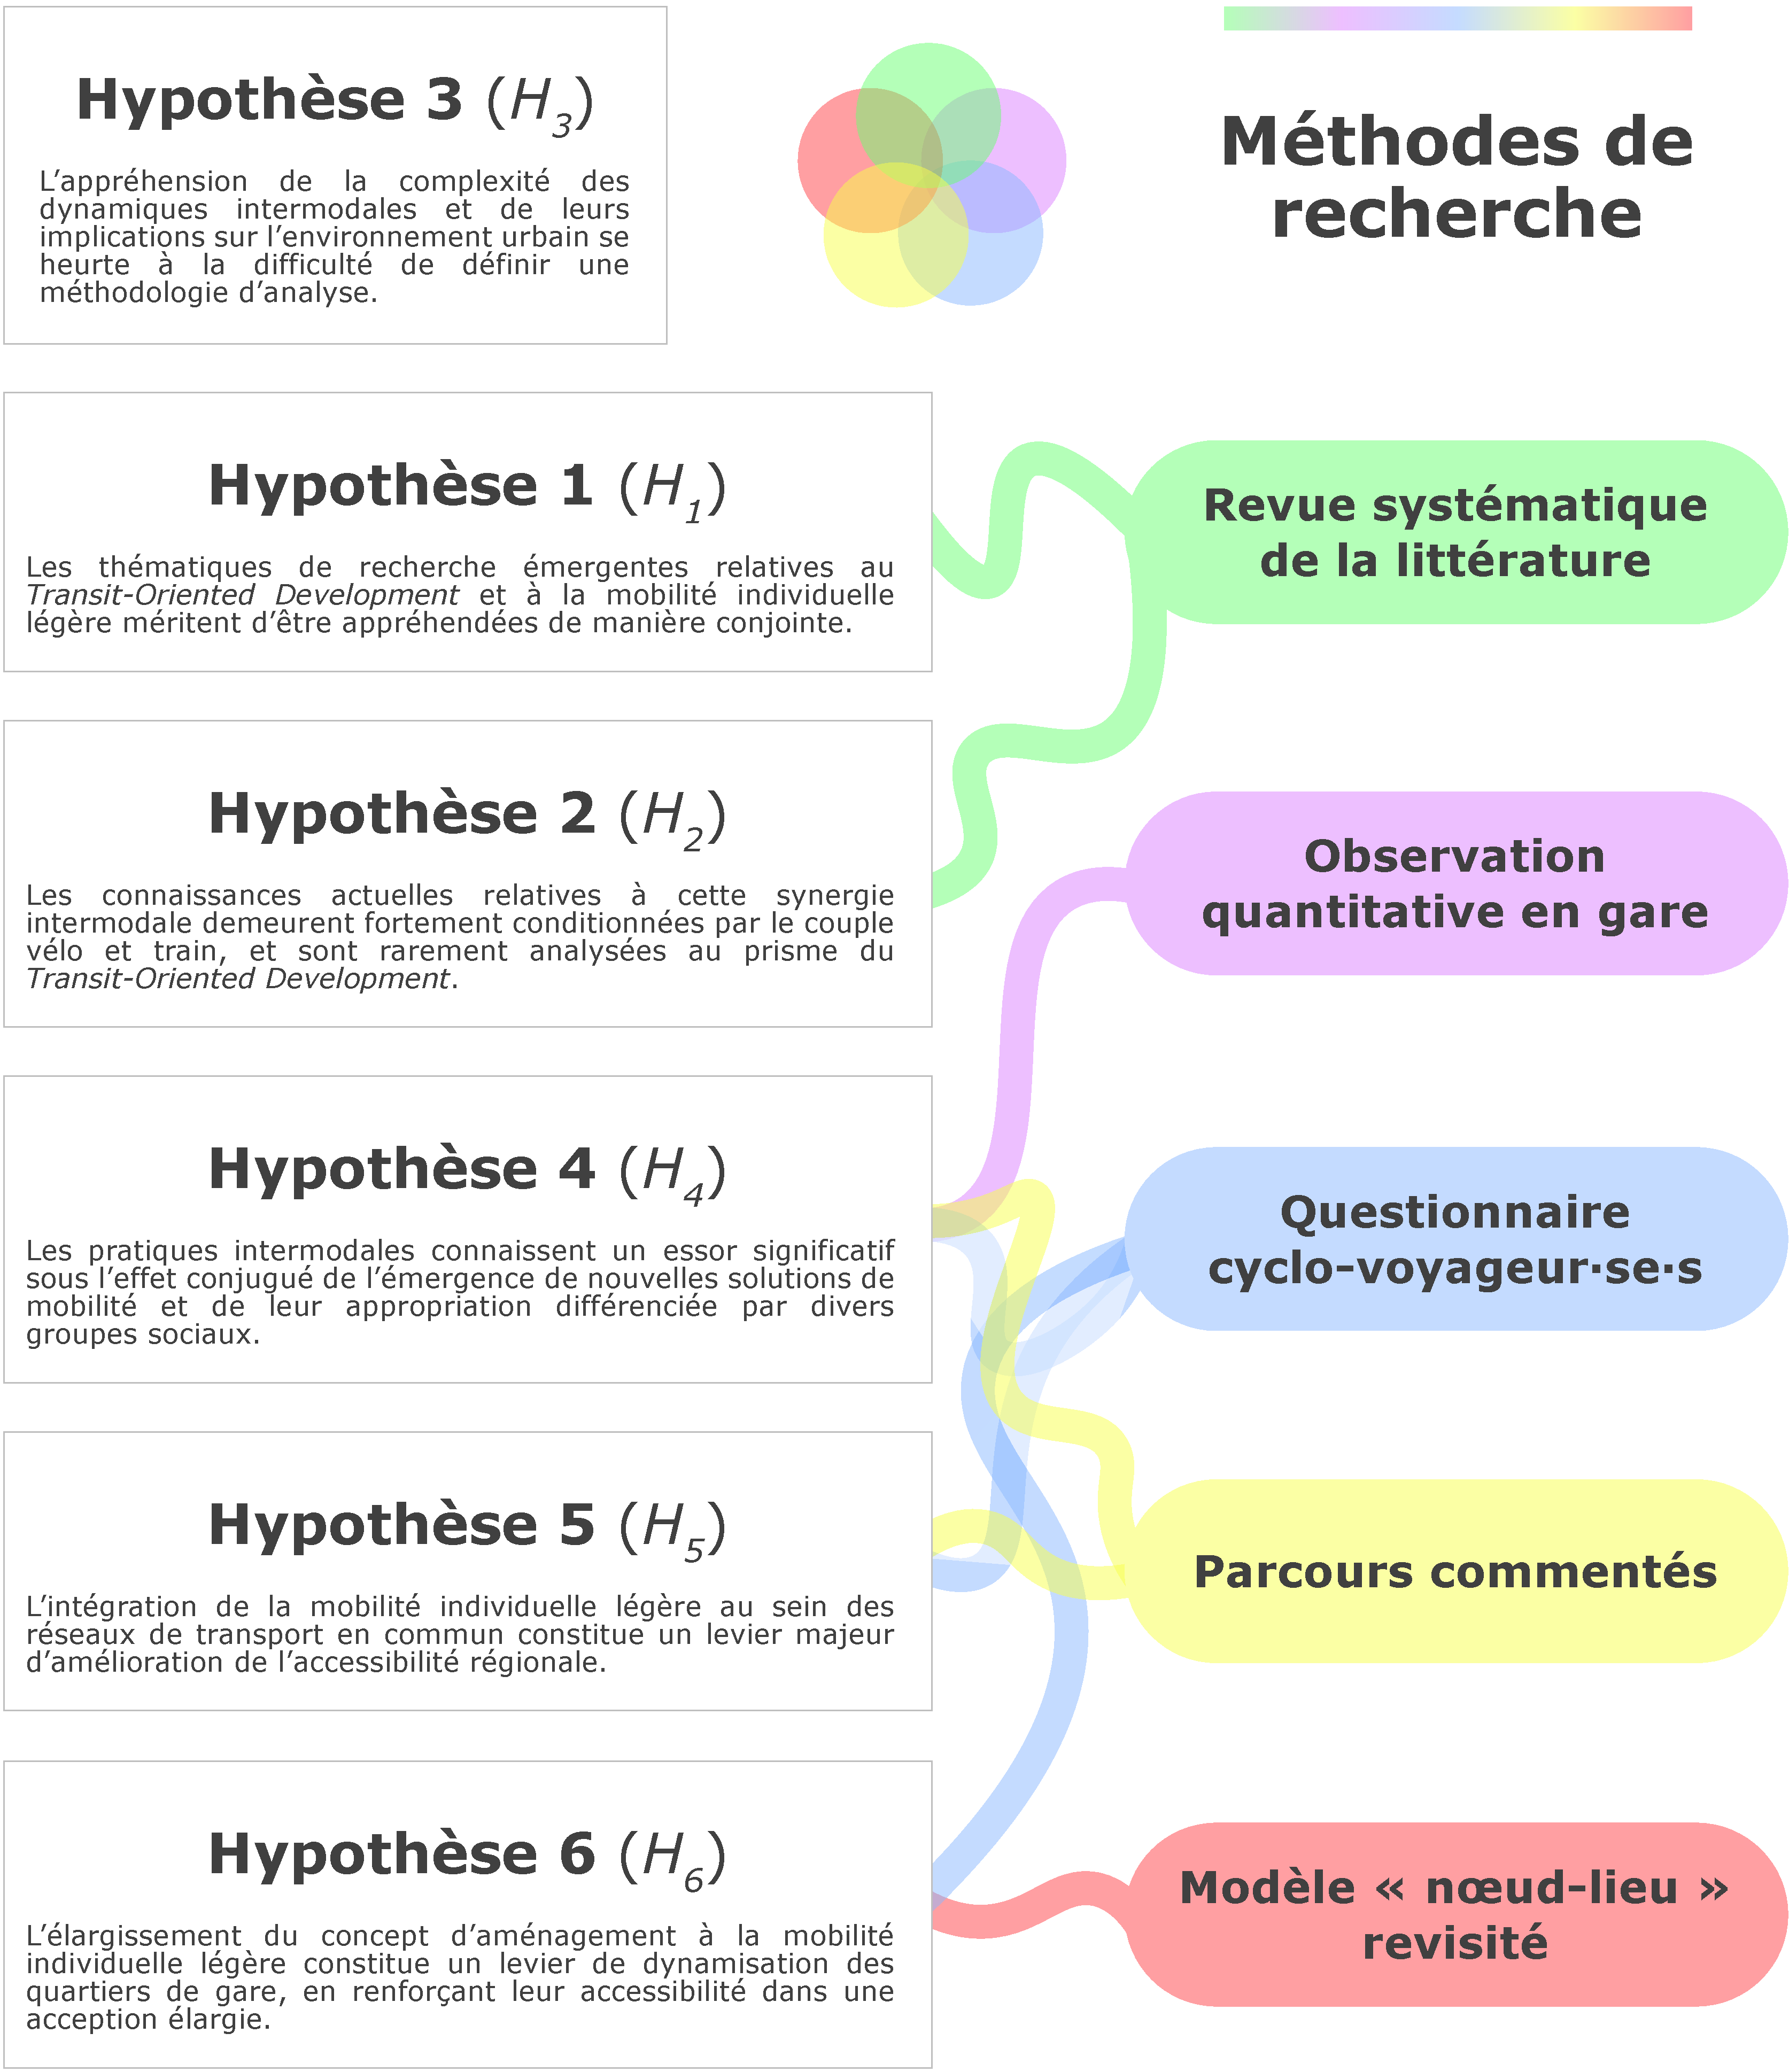
\includegraphics[width=1\columnwidth]{src/Figures/Introduction/FR_Methodologie_hypotheses.pdf}}
        \vspace{5pt}
        \begin{flushright}\scriptsize{
        Auteur~: \textcolor{blue}{Dylan Moinse (2025)}
        }\end{flushright}
    \end{figure}

    % Méthodologie
La méthodologie retenue repose, en premier lieu, sur le besoin de synthétiser les travaux et les connaissances existants, relatifs à la problématique de recherche. À cette fin, une \acrfull{RSL} a été conduite sur les études s’apparentant aux contours du \acrshort{B-TOD} et du \acrshort{M-TOD}, dans la continuité des \hyperref[hypothese-1]{hypothèses~\(H_1\)} et \hyperref[hypothese-2]{\(H_2\)} (page~\pageref{hypothese-2}). S'ensuit une exploration de terrain sous la forme d’une observation quantitative, visant à caractériser le phénomène émergent de la connexion nodale réalisée à l'aide de la mobilité individuelle légère, en adéquation avec l'\hyperref[hypothese-4]{hypothèse~\(H_4\)} (page~\pageref{hypothese-4}). Cette enquête est complétée par la conduite d'entretiens mobiles, le parcours commenté, venant enrichir l'investigation en accédant à la \gls{perception} des usager·ère·s et d'affiner la compréhension de leurs pratiques intermodales. Un troisième type d’enquête repose sur un questionnaire adressé aux cyclo-voyageur·se·s, destiné à représenter les déplacements intermodaux en vue d’identifier les territoires fréquentés et vécus à proximité des pôles d’échange, dans le prolongement de l'\hyperref[hypothese-5]{hypothèse~\(H_5\)} (page~\pageref{hypothese-5}). Enfin, une modélisation spatiale a été entreprise, dans le but de revisiter l'outil \Guillemets{nœud-lieu}, usuellement appliqué dans les travaux sur le \acrshort{TOD}. Cette modélisation permet de saisir les implications de l’intégration de la mobilité individuelle légère et d’identifier ses interactions avec l’environnement urbain, en appui sur l'\hyperref[hypothese-6]{hypothèse~\(H_6\)} (page~\pageref{hypothese-6}).%%Rédigé%%

% --- %
    % *.5. Annonce du plan
    \needspace{1\baselineskip} % Réserve de l'espace
\section*{Structure de la thèse
    \label{introduction-generale:annonce-plan}
    }
    \addcontentsline{toc}{section}{Structure de la thèse}
    %\markboth{Annonce du plan}{}
    \markright{Annonce du plan}{}

    % Introduction
Cette thèse se structure en trois parties et six chapitres, suivant une progression logique qui permet d’explorer les fondements théoriques, les enjeux et les implications de l’intégration de la mobilité individuelle légère dans le modèle du \acrshort{TOD} (voir le \hyperref[fig-introduction:structure-these]{schéma~\ref{fig-introduction:structure-these}}, page~\pageref{fig-introduction:structure-these}). Alternant entre approche conceptuelle, état de l’art, cadre méthodologique, étude empirique et modélisation prospective, elle aboutit à la proposition d’un modèle renouvelé~: un \acrfull{M-TOD}. L’argumentaire développé repose sur trois axes majeurs~: (i) une compréhension approfondie des usages et des comportements liés à la mobilité individuelle légère dans une perspective intermodale~; (ii) une analyse multicritère du potentiel d’accueil des territoires en fonction de leur capacité à intégrer ces nouvelles formes de mobilité~; et (iii) une interrogation sur le rôle de l’action publique dans l’aménagement et la structuration de ces pratiques au sein des politiques de transport et d’urbanisme. En parallèle, trois niveaux d’analyse progressifs et multiscalaires sous-tendent cette réflexion~: (i) l’examen des dynamiques de la demande intermodale~; (ii) l’évaluation de l’accessibilité intermodale, considérée sous l’angle de la performance des réseaux, des ressources disponibles, des contraintes temporelles et des caractéristiques individuelles~; (iii) ainsi que l’analyse des interactions entre transport et urbanisme dans un contexte d'intégration modale. La structuration de cette recherche qui traduit la démarche scientifique adoptée peut être synthétisée comme suit~: \textsl{synthétiser et repenser} (voir la \hyperref[part1:titre]{première partie}, page~\pageref{part1:titre})~; \textsl{représenter et comprendre} (voir la \hyperref[part2:titre]{deuxième partie}, page~\pageref{part2:titre})~; puis \textsl{anticiper et orienter} (voir la \hyperref[part3:titre]{troisième partie}, page~\pageref{part3:titre}).%%Rédigé%%

    % Figure structure de la thèse
    \begin{figure}[h!]\vspace*{4pt}
        \caption{Structure générale de la recherche doctorale}
        \label{fig-introduction:structure-these}
        \centerline{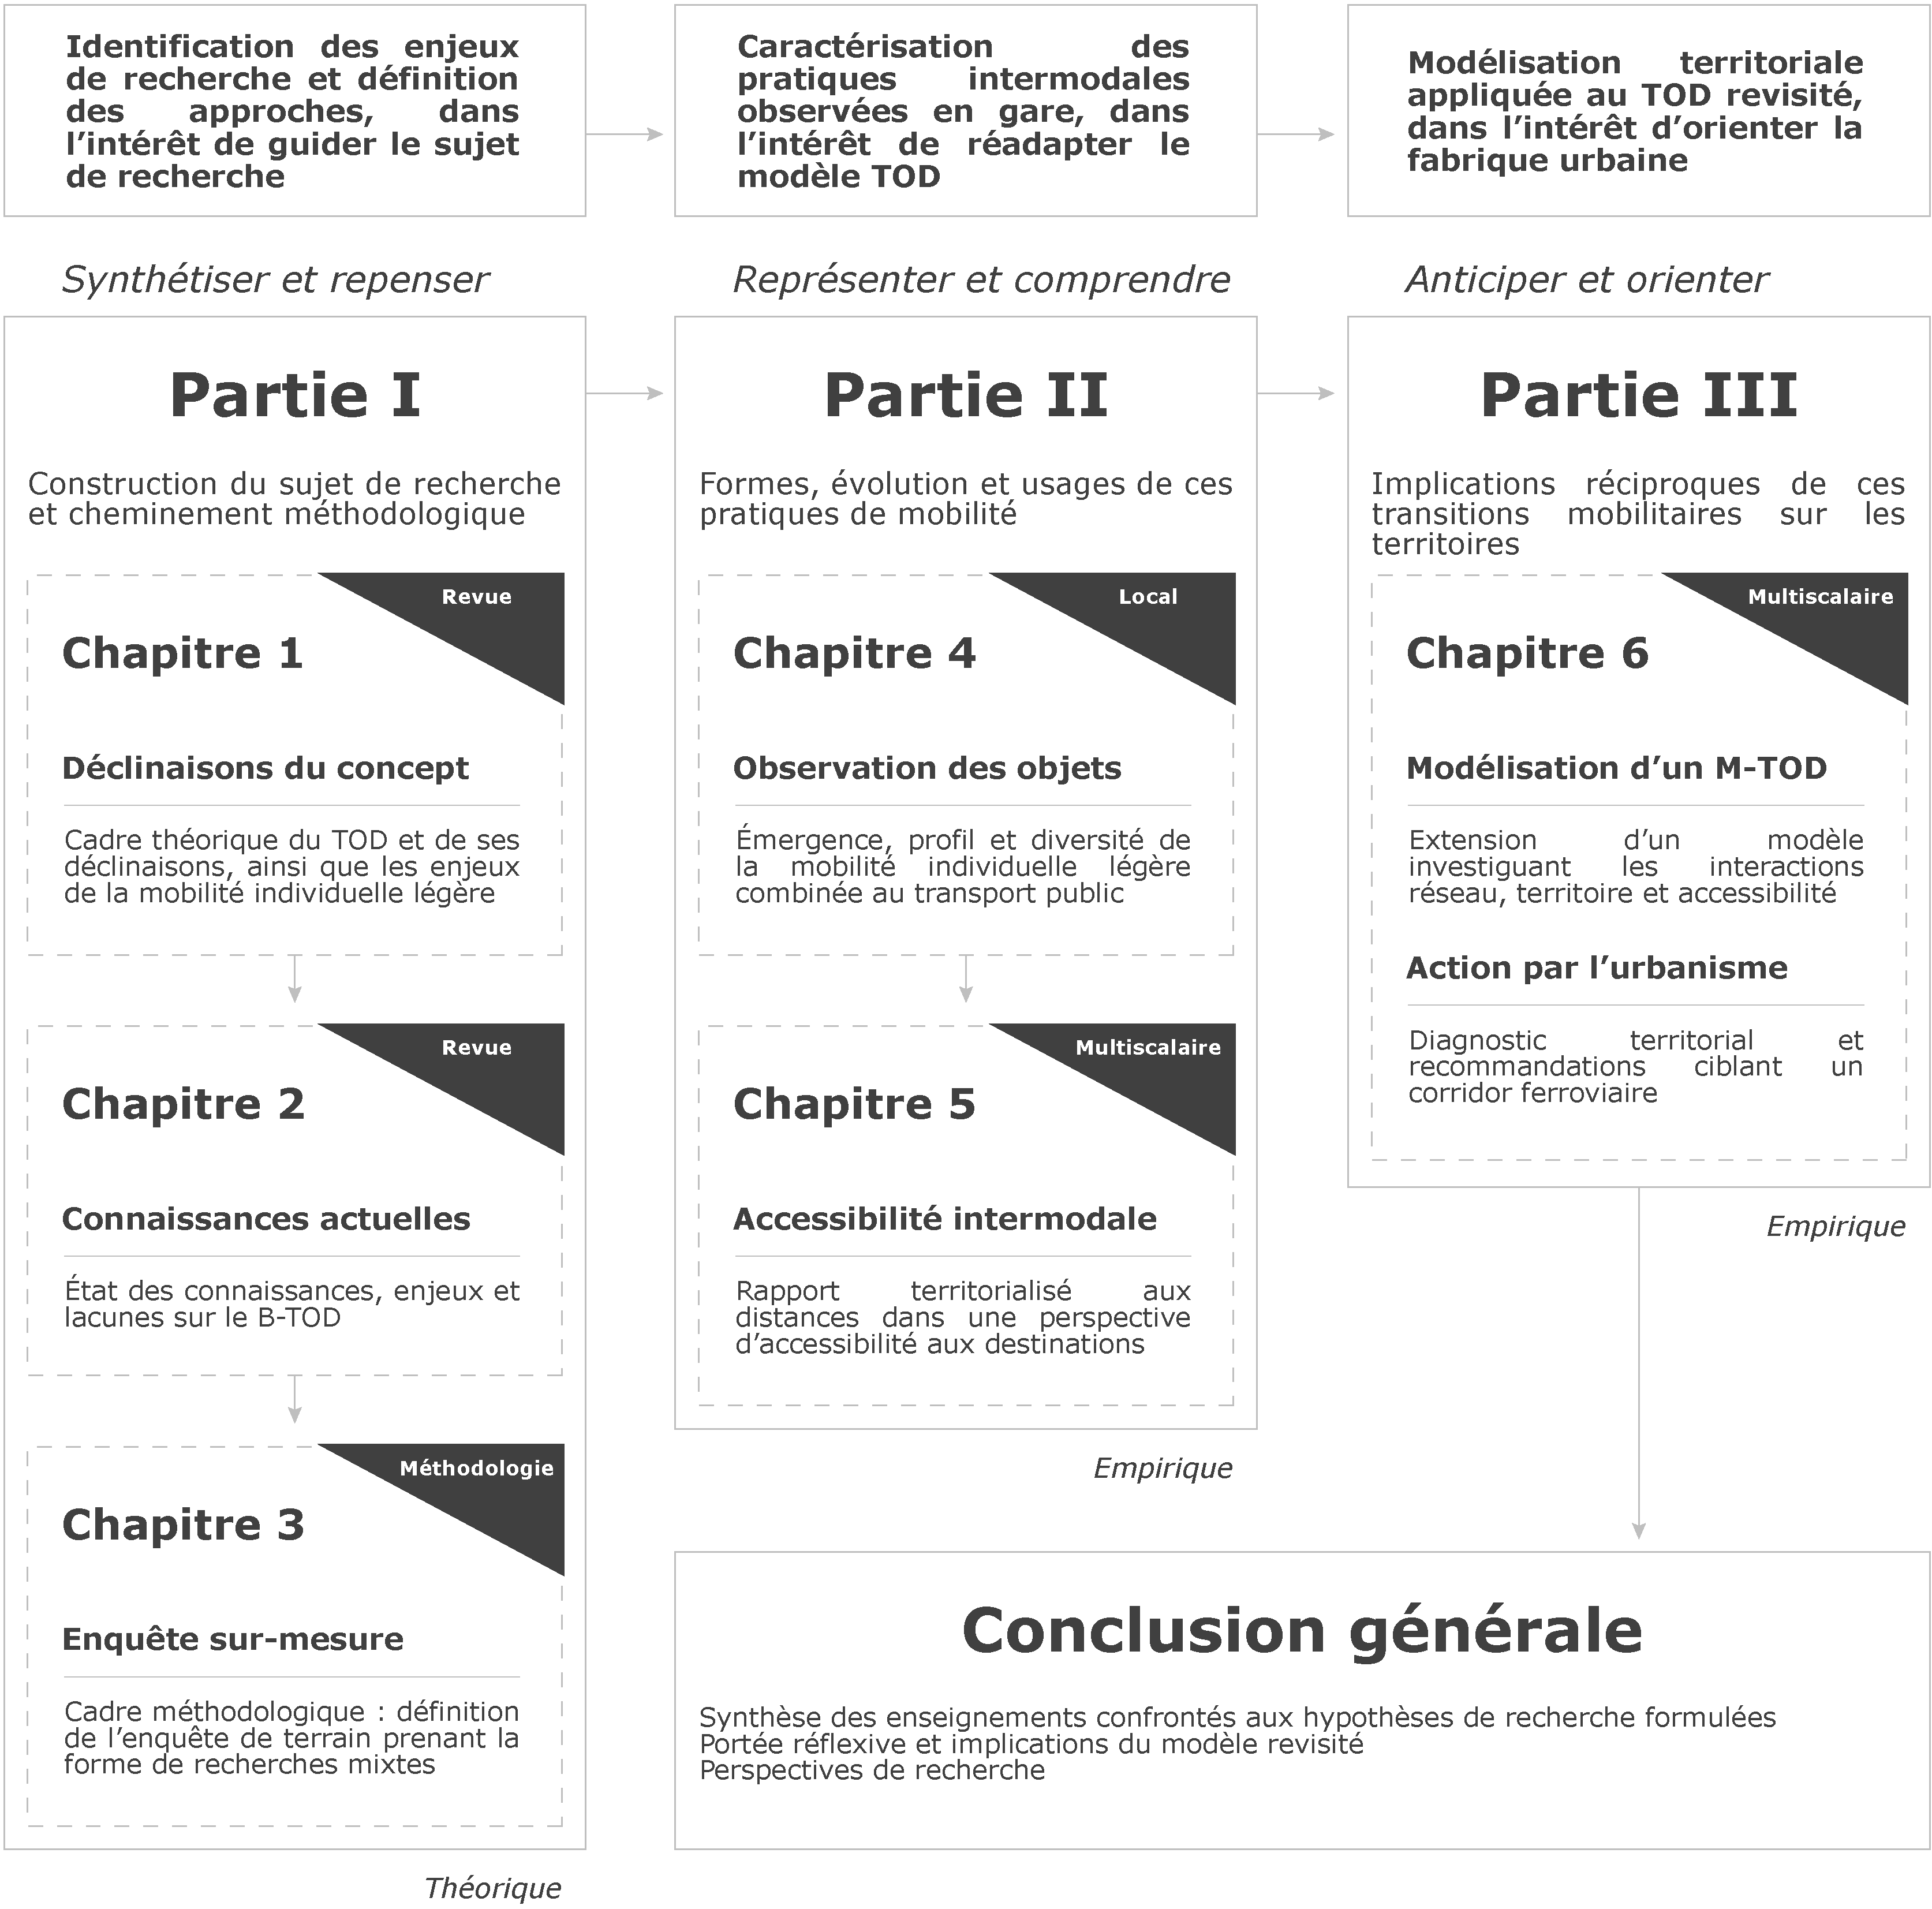
\includegraphics[width=1\columnwidth]{src/Figures/Introduction/FR_Structure_these.pdf}}
        \vspace{5pt}
        \begin{flushright}\scriptsize{
        Auteur~: \textcolor{blue}{Dylan Moinse (2023)}
        }\end{flushright}
    \end{figure}

    % *.5.1. Annonce du plan : partie 1
    \needspace{1\baselineskip} % Réserve de l'espace
\subsection*{Première partie~: \textsl{Synthétiser et repenser}
    \label{introduction-generale:annonce-plan-1}
    }

    % Chapitre 1
\hyperref[chap1:titre]{Le premier chapitre} (page~\pageref{chap1:titre}) pose les bases théoriques de cette recherche en définissant les concepts fondamentaux qui structureront l’argumentation. Il s’attarde tout d’abord sur les principes fondateurs du \acrshort{TOD}, en retraçant son évolution et ses diverses adaptations conceptuelles et opérationnelles. Ce modèle d’aménagement, pensé comme une alternative au système auto-centré, vise à structurer l’urbanisation autour des infrastructures de transport en commun. Toutefois, son application révèle des limites dans certains contextes, notamment dans les territoires périurbains où les distances d’accès aux stations de transport public constituent un frein majeur à son efficacité. C’est dans cette perspective que s’inscrit l’analyse de la mobilité individuelle légère, définie ici comme un ensemble de véhicules incluant le vélo et ses variantes, ainsi que la trottinette et d’autres engins de déplacement. Ces solutions émergent comme un levier stratégique susceptible de pallier les insuffisances du \acrshort{TOD} conventionnel en améliorant l’accessibilité aux nœuds, sous l'angle des \Guillemets{premiers et derniers kilomètres} du transport public. Ce chapitre explore ainsi la montée en puissance des cycles dans la mobilité quotidienne et leur prise en compte progressive dans les politiques d’aménagement. Il s’attache ensuite à examiner les opportunités qu’implique l’intégration de la mobilité individuelle légère dans la pensée du \acrshort{TOD}, en interrogeant ses implications en matière de proximité géographique et d’intermodalité. Enfin, il s’achève sur une revue critique de la littérature, mettant en évidence les lacunes théoriques et les potentiels d’un modèle élargi intégrant ces nouvelles articulations entre mobilité et urbanisme, qui viennent justifier l’investigation menée dans cette thèse (\hyperref[objectif-1]{objectif~\(O_1\)}, page~\pageref{objectif-1}).%%Rédigé%%

    % Chapitre 2
\hyperref[chap2:titre]{Le deuxième chapitre} (page~\pageref{chap2:titre}) prolonge la réflexion engagée sur l’évolution du \acrshort{TOD} en approfondissant l’état des connaissances sur ses déclinaisons intégrant la mobilité individuelle légère, en particulier le \acrshort{B-TOD} et le \acrshort{M-TOD}. Il dresse un état de l’art sur l’articulation entre le vélo, la micro-mobilité et le transport public, en questionnant ces interactions à l'interface des systèmes de mobilité et de l'organisation territoriale. S’appuyant sur une \acrfull{RSL}, ce chapitre mobilise une approche scientométrique permettant d’identifier les dynamiques géographiques, temporelles et institutionnelles structurant ces modèles d'urbanisme. Cette étude soutient l’essor récent des recherches consacrées à ces thématiques et l’émergence de nouveaux outils méthodologiques, en particulier l’exploitation de la \textsl{Big Data} et des modèles d'analyse géostatistiques. Elle identifie les principaux déterminants urbains influençant les comportements de mobilité et évalue les gains d’accessibilité induits par l’intégration de la mobilité individuelle légère dans les stratégies \acrshort{TOD}\textcolor{blue}{s}. Sur la base de ces éléments, ce chapitre définit les assises théoriques et méthodologiques sur lesquelles repose l'investigation empirique conduite dans les prochains chapitres (\hyperref[objectif-2]{objectif~\(O_2\)}, page~\pageref{objectif-2}).%%Rédigé%%

    % Chapitre 3
\hyperref[chap3:titre]{Le troisième chapitre} (page~\pageref{chap3:titre}) marque l'entrée sur le terrain d'étude de la thèse en cherchant à évaluer l'intégration de la mobilité individuelle légère dans le modèle urbain. Il expose le cadre méthodologique adopté pour mener cette enquête. Ce chapitre prend part à une réflexion sur le positionnement épistémologique de la recherche, en justifiant l’adoption de recherches mixtes, combinant approches quantitatives et qualitatives. Cette méthodologie permet d’appréhender la complexité des comportements de mobilité ainsi que leurs rapports et leurs effets sur l'accessibilité territoriale, en croisant différentes sources d’information. Cette démarche, décrivant les choix méthodologiques, les outils de collecte et de traitement des données ainsi que la construction des terrains, pose le socle analytique qui guide l’interprétation des résultats dans les parties qui suivent (\hyperref[objectif-3]{objectif~\(O_3\)}, page~\pageref{objectif-3}).%%Rédigé%%

    % *.5.2. Annonce du plan : partie 2
    \needspace{1\baselineskip} % Réserve de l'espace
\subsection*{Deuxième partie~: \textsl{Représenter et comprendre}
    \label{introduction-generale:annonce-plan-2}
    }

    % Chapitre 4
\hyperref[chap4:titre]{Le quatrième chapitre} (page~\pageref{chap4:titre}) constitue la première phase de l’analyse empirique en s’attachant à l’étude des pratiques intermodales associées à la mobilité individuelle légère, qui s'inscrivent dans les quartiers de gare. Il vise, d’une part, à quantifier l’ampleur du phénomène, en mesurant la part modale des modes de transfert dans les chaînes de déplacement impliquant les transports en commun. D’autre part, il cherche à mieux définir le corpus de cyclo-voyageur·se·s et à identifier les facteurs déterminants de leurs choix modaux, en tenant compte de leurs caractéristiques individuelles, de leurs perceptions, ainsi que de leur rapport à l’environnement urbain. Ce chapitre met en lumière les arbitrages réalisés par les usager·ère·s dans leur organisation quotidienne des déplacements intermodaux et souligne le rôle des agencements territoriaux en tant que facteurs structurants de ces pratiques émergentes. Il met en évidence les conditions favorisant leur essor et prépare ainsi l’analyse spatiale du chapitre suivant, en questionnant le rôle de l’accessibilité et des configurations urbaines comme catalyseurs de ces comportements (\hyperref[objectif-4]{objectif~\(O_4\)}, page~\pageref{objectif-4}).%%Rédigé%%

    % Chapitre 5
Sur la base des résultats exploratoires obtenus, \hyperref[chap5:titre]{Le cinquième chapitre} (page~\pageref{chap5:titre}) se focalise sur les gains d'accessibilité générés par ces synergies modales. Il interroge la manière dont ces pratiques intermodales transforment l’accessibilité aux gares et participent à la reconfiguration des quartiers environnants, en redéfinissant les périmètres d’influence des nœuds. Il s'agit principalement d'évaluer l'apport de la mobilité individuelle légère dans l'extension des bassins de desserte des arrêts de transport en commun, ainsi que les bénéfices en termes d'accès régional aux destinations. La projection des itinéraires empruntés met en relief les parcours privilégiés et les facteurs qui influencent ces choix. Cette réflexion conduit à une lecture renouvelée des périmètres fonctionnels des quartiers de gare, en montrant comment l’intégration de la mobilité individuelle légère peut modifier leur organisation spatiale et renforcer leur attractivité en tant que lieu stratégique (\hyperref[objectif-5]{objectif~\(O_5\)}, page~\pageref{objectif-5}).%%Rédigé%%

    % *.5.3. Annonce du plan : partie 3
    \needspace{1\baselineskip} % Réserve de l'espace
\subsection*{Troisième partie~: \textsl{Anticiper et orienter}
    \label{introduction-generale:annonce-plan-3}
    }

    % Chapitre 6
\hyperref[chap6:titre]{Le sixième chapitre} (page~\pageref{chap6:titre}) propose une formalisation du \acrshort{M-TOD}, conçu comme une extension du \acrshort{TOD} veillant à pleinement intégrer les proximités géographiques promises par l'usage de la marche combinée et de la mobilité individuelle légère. À partir des enseignements tirés, ce chapitre engage une modélisation du \acrshort{M-TOD}, de manière à définir ses principes directeurs, ses conditions de mise en œuvre, ainsi que les leviers d’action à activer pour favoriser son développement et maximiser ses bénéfices. La modélisation proposée permet notamment de prédire la fréquentation des gares en fonction des agencements territoriaux de chacun des quartiers de gare examinés, et des échelles d’accessibilité piétonnière et cyclable dans le périmètre régional étudié. Une classification des gares et de leurs bassins de desserte est alors établie, permettant d’identifier les pôles urbains stratégiques détenant un potentiel de mise en application du \acrshort{TOD} et du \acrshort{M-TOD}, ainsi que ceux pour lesquels des investissements et des améliorations sont à envisager afin de renforcer leur rôle dans un système de mobilité alternatif global. Enfin, ce chapitre s’ouvre sur la production d'un diagnostic territorial en formulant une série de recommandations stratégiques, appliquées à une étude de cas portant sur un corridor ferroviaire (\hyperref[objectif-6]{objectif~\(O_6\)}, page~\pageref{objectif-6}).%%Rédigé%%

    % ___________________________________________
    % Sous-bibliographie
    \newpage
    %\sectionheader{Sous-bibliographie de l'introduction générale}
    \begingroup
    \renewcommand{\bibfont}{\scriptsize}
\printbibliography[segment=\therefsegment, heading=subbibintoc, title={Sous-bibliographie de l'introduction générale}, label=introduction:bibliographie]
    \endgroup
    \end{refsegment}